% PWM messen: Input-Capture mit 2 Kanaelen (CCR1 = Periode, CCR2 = Pulsdauer)
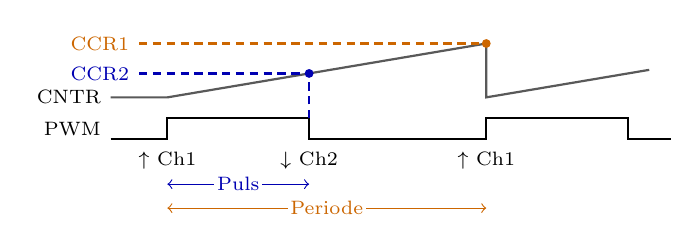
\begin{tikzpicture}[x=0.9cm,y=0.38cm,font=\scriptsize]
  % PWM-Signal
  \draw[thick] (0,0)--(0.8,0)--(0.8,0.7)--(2.8,0.7)--(2.8,0)--(5.3,0)--(5.3,0.7)--(7.3,0.7)--(7.3,0)--(7.9,0);
  \node[anchor=east] at (0,0.35) {PWM};
  % Counter (Saegezahn, Reset bei steigender Flanke)
  \draw[thick,gray!70!black] (0,1.4)--(0.8,1.4)--(5.3,3.2)--(5.3,1.4)--(7.3,2.2)--(7.6,2.32);
  \node[anchor=east] at (0,1.4) {CNTR};
  % CCR1 (Periode)
  \draw[orange!80!black,densely dashed,thick] (0.4,3.2)--(5.3,3.2);
  \fill[orange!80!black] (5.3,3.2) circle (1.6pt);
  \node[orange!80!black,anchor=east] at (0.4,3.2) {CCR1};
  % CCR2 (Pulsdauer)
  \draw[blue!70!black,densely dashed,thick] (0.4,2.2)--(2.8,2.2);
  \draw[blue!70!black,densely dashed,thick] (2.8,0.7)--(2.8,2.2);
  \fill[blue!70!black] (2.8,2.2) circle (1.6pt);
  \node[blue!70!black,anchor=east] at (0.4,2.2) {CCR2};
  % Flanken
  \node[anchor=north] at (0.8,-0.1) {$\uparrow$ Ch1};
  \node[anchor=north] at (2.8,-0.1) {$\downarrow$ Ch2};
  \node[anchor=north] at (5.3,-0.1) {$\uparrow$ Ch1};
  % Masse
  \draw[<->,blue!70!black] (0.8,-1.5)--(2.8,-1.5) node[midway,fill=white,inner sep=1pt] {Puls};
  \draw[<->,orange!80!black] (0.8,-2.3)--(5.3,-2.3) node[midway,fill=white,inner sep=1pt] {Periode};
\end{tikzpicture}
